\section{Leader/Followers}

The Leader/Followers architectural pattern provides an efficient concurrency model where multiple threads take turns sharing a set of event sources in order to detect, demultiplex, dispatch, and process service requests that occur on the event sources.

\subsection{Kontext}

Eine eventbasierte Applikation, in welcher mehrere Service Requests von mehreren Event-Quellen gleichzeitig auftreten und effizient von mehreren Threads abgearbeitet werden müssen.

\subsection{Problem}

Multithreading wird oft verwendet, um mehrere Events nebenläufig zu verarbeiten. Es ist jedoch schwierig, das auch performant zu implementieren.
Folgende Punkte müssen eingehalten werden:
\begin{itemize}
	\item Das Demultiplexen von Event-Quelle nach Worker-Thread muss effizient gestaltet werden. Ein Thread pro Event-Quelle skaliert oft nicht effizient.
	\item Der Overhead, welcher durch Nebenläufigkeit generiert wird, wie Context-Switching, Synchronisation, Cache-Kohärenz-Management, sollte minimiert werden. Insbesondere Nebenläufigkeitsmodelle, welche bei Übergabe von Daten dynmisch Speicher allozieren, wirken sich negativ auf die Performance aus.
	\item Race-Conditions müssen verhindert werden, wenn mehrere Threads auf die gleichen Event-Quellen zugreifen.
\end{itemize}

\subsection{Lösung}

Einen Thread-Pool-Mechanismus erstellen, welcher sich Event-Quellen effizient teilt, indem ein Thread nach dem anderen je einen Event synchron an einen Applikations-Service ausliefert. Es wartet immer nur ein Thread (der Leader), auf einen Event. Die anderen Threads (Follower), reihen sich in eine Queue ein und warten. Sobald der Leader einen Event detektiert, wählt er zuerst den nächsten Leader aus den Followern aus, und liefert den Event dann als Processing-Thread einem Event-Handler aus, welcher das applikations-spezifische Event-Handling im Processing-Thread durchführt. Sobald der Thread mit dem Processing fertig ist, prüft er, ob es noch einen Leader gibt. Falls nicht, wird er der Leader. Andernfalls legt er sich wieder schlafen und wartet, bis er zum neuen Leader ernannt wird.


\subsection{Struktur}

\begin{itemize}
	\item \emph{Handles} werden vom Betriebssystem zur Identifikation der Event-Quellen zur Verfügung gestellt (i.e. ein file handle).
	\item Ein \emph{Handle Set} erlaubt auf meherern Handles auf einen Event zu warten.
	\item Ein \emph{Event Handler} spezifiziert das Interface für den applikations-spezifischen Code.
	\item Der \emph{Thread pool} managed die Threads welche eine Protokoll zur Koordination implementieren (Leader/Follower-Detection). Die Threads warten auf einen Event von einem Handle aus ihrem Handle Set. Sobald ein Event auftritt, wählt der Thread den nächsten Leader aus und liefert den Event dann einem Event Handler aus.
\end{itemize}

\subsubsection*{Klassendiagramm}

\begin{figure}[H]
	\centering
	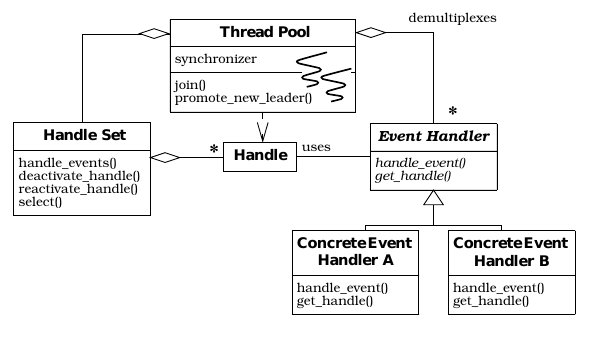
\includegraphics[width=\textwidth]{content/posa2/images/leaderFollowerStructure.jpeg}
	\caption{leaderFollowerStructure}
\end{figure}


\subsubsection*{Sequenzdiagramm}


\begin{figure}[H]
	\centering
	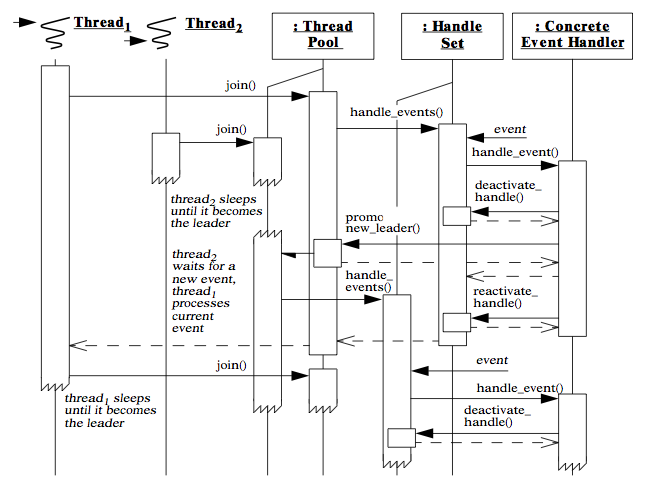
\includegraphics[width=\textwidth]{content/posa2/images/leaderFollowersSequenceDiagram.png}
	\caption{Leader/Followers Sequence Diagram}
\end{figure}


\subsubsection*{Zustandsdiagramm}


\begin{figure}[H]
	\centering
	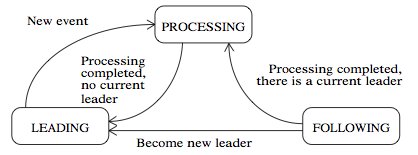
\includegraphics[width=\textwidth]{content/posa2/images/leaderFollowersStateDiagram.png}
	\caption{Leader/Followers State Diagram}
\end{figure}


